\documentclass[../ASSD_TP2.tex]{subfiles}
\begin{document}
\section*{S\'intesis Aditiva}
\subsection*{Introducci\'on}
La s\'intesis aditiva recrea una señal de sonido mediante la suma de senoidales de diferentes frecuencias (la frecuencia fundamental y sus armonicos) haciendo uso de las series de Fourier. Adem\'as, para que el sonido que sintetiza sea lo mas parecido al de un instrumento real, se debe dar la forma a cada senoidal con una envolvente, que esta depende de cada instrumento.

\subsection*{Teor\'ia}
Para recrear una señal hay que hacer uso de la serie de Fourier (comentado anteriormente), entonces
\begin{align*}
  S(x) &= \sum_{n=0}^{+\infty} a_n*sin(2*\pi*n + \phi) \\
\end{align*}
Esta serie es la ideal, ya que se extiende hasta el infinito, pero para este caso, basta con tomar un $N = 20.000$ debido a que es la frecuencia hasta la que llega el rango audible, frecuencias m\'as altas que esas no se escuchar\'ian, por lo cual, no aportaria nada al sonido final. Por lo tanto
\begin{align*}
  S(x) &= \sum_{n=0}^{20.000} a_n*sin(2*\pi*n + \phi) \\
\end{align*}
Los t\'erminos $a_n$ son los coeficientes de la serie de Fourier, que son los que determinan cual es la amplitud de cada frecuencia.
Como se puede apreciar, esta señal es infinita en el tiempo, por lo tanto, hay que multiplicarle una funcion que dependa del tiempo, para que deje de serlo. Cada instrumento posee una diferente.
\begin{align*}
  S(x) &= \sum_{n=0}^{20.000}a(t)* a_n*sin(2*\pi*n*t + \phi) \\
\end{align*}
\subsection*{Aplicaci\'on}
\subsubsection*{Coeficientes de Fourier}
Para hallar los coeficientes de la serie de Fourier, hay que aplicarle la trasformada r\'apida de Fourier (FFT) y aplicandole el m\'odulo a este resultado, se obtiene la amplitud que tiene cada frecuencia, esta amplitud es $a_n$.
Por otra parte, la fase tambien es simple de encontrarla, aunque se llego a la conclusi\'on de que no afecta considerablemente la calidad de sonido, entonces no se utilizo la fase, ya que seria mucho tiempo de procesamiento para el cambio que hace.
Para obtener los $a_n$, lo que se hizo fue encontrar los picos de la FFT, porque tomar todos los valores de esta seria muy ineficiente en terminos de tiempo de procesamiento.
La siguiente figura, muestra la FFT de la señal original, con los picos hallados.

\begin{figure}[H]
\centering
  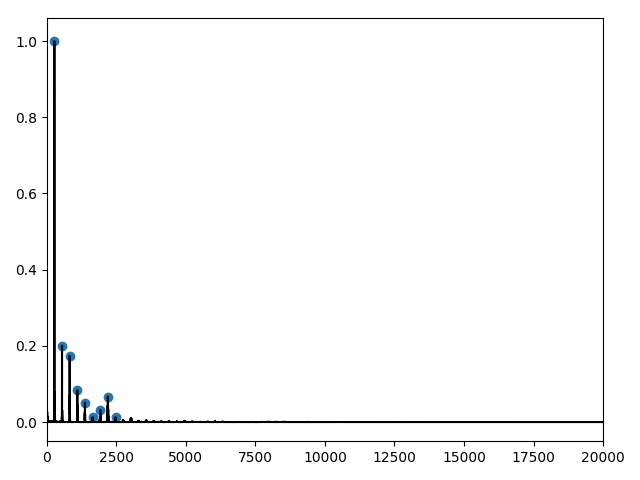
\includegraphics[width=0.6\linewidth]{fft_with_peaks.png}
  \caption{FFT de la señal de un cello con los picos}
  \label{fig:fft}
\end{figure}

\subsubsection*{Envolvente}
Para realizar la envolvente, se intentaron varios m\'etodos, como el detector de picos y valor RMS, entre otros. El que se termino utilizando fue el detector de picos y luego se interpolaron esos picos, para que la envolvente sea mas suave y no genere distorsi\'on.
\begin{figure}[H]
\centering
  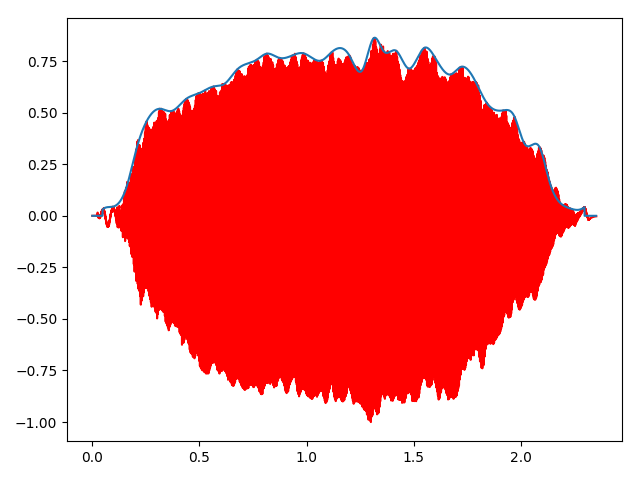
\includegraphics[width=0.6\linewidth]{envolvente.png}
  \caption{señal de entrada (rojo) con la envolvente (azul)}
  \label{fig:envolvente}
\end{figure}
Como se ve en la figura, la envolvente sigue perfectamente a la señal, lo cual har\'a que el sonido a la salida sea mas claro.

\subsection*{S\'intesis de los Instrumentos}
El programa fue realizado en principio para un Cello, pero luego se le fueron cargando otros instrumentos, los cuales tambien funcionaban muy bien. Estos instrumentos fueron, piano, tuba, saxo y violin. La tuba y el cello fueron los intrumentos que mejor sonaron, seguidos por el saxo y el violin.
El instrumento que peor son\'o fue la guitarra, que la sintesis hecha, no tenia sonido de guitarra.

\subsection*{Conclusi\'on}
El programa implementado se comport\'o muy bien con los instrumentos mencionados anteriormente, y el tiempo de procesamiento fue muy bueno. Es cierto que posee ciertas limitaciones con respecto a algunos instrumentos, como por ejemplo la guitarra. 

\end{document}
